%\documentclass[12pt]{article}
%\usepackage[latin1]{inputenc}
%\usepackage[spanish]{babel}
%\usepackage{latexsym}
%\usepackage{amssymb}
%\usepackage{amsmath}

%\setlength{\textwidth}{15cm}

%\newtheorem{ejem}{Ejemplo}
%\newtheorem{teor}{Teorema}
%\begin{document}

\chapter{MARCO TEÓRICO}
\section{DEFINICIONES BÁSICAS}
\subsection{EL PROCESO DE DESARROLLO DE SOFTWARE}

El proceso de desarrollo de software tiene como propósito la producción eficaz y eficiente de un producto software que reúna los requisitos del cliente. Este proceso es intensamente intelectual, afectado por la creatividad y juicio de las personas involucradas. Aunque un proyecto de desarrollo de software es equiparable en muchos aspectos a cualquier otro proyecto de ingeniería, en el desarrollo de software hay una serie de desafíos adicionales, relativos esencialmente a la naturaleza del producto obtenido. \\

En aspectos generales sin enfocarnos al concepto de cada metodología utilizada para realizar esta labor, podemos ver que nos enfocamos en la evolución del código.\\

Ya sea que trabajemos en grupo o de forma individual, esta actividad se comienza con una hoja en blanco y una idea en la cabeza, que a medida que progresamos, va tomando forma.
Enfocandonos desde el punto de vista del código realizado durante este proceso, al principio arrancamos con un directorio vacío, en el cual vamos escribiendo, construyendo nuestro software
de forma incremental e iterativa, corrigiendo nuestros propios errores a medida que aparecen, y agregando cosas nuevas cuando se nos place.\\

Nuestro código va evolucionando, cambiando con iteraciones pequeñas que nosotros vamos introduciendo por diversos motivos como, correcciones o características nuevas en el software.
Estos cambios realizados en el código son de manera organizada y ordenada, debido a que corresponden a alguna construcción mental nuestra, porque cuando nosotros pensamos en implementar algo o corregir un bug\footnote{Un bug es un mal funcionamiento de un elemento de software: que un programa haga cosas no queridas, o que no haga las cosas que debería.}, lo tenemos en mente como una unidad, como un objetivo bastante independiente de como se representa en el código fuente; y nosotros pensamos en que cambios le tenemos que realizar para lograr ese objetivo propuesto.

\subsection{GRUPOS DE TRABAJO EN EL DESARROLLO DE SOFTWARE}

En la actividad de desarrollo de software con frecuencia los desarrolladores son organizados en grupo, independientemente de que metodología empleen. Surgiendo la suma necesidad de coordinar el trabajo, no solo por una cuestión natural sino también como mecanismo para optimizar los recursos.\\
Por eso, para desarrollar en grupo es imprescindible la buena comunicación y el entendimiento entre los pares. Esto implica que, en general los desarrollos se dan de forma coordinada (ya sea de manera horizontal o vertical, independientemente del mecanismo que se elija explícita o implícitamente para ello) al menos en un nivel social, las tareas se reparten y los cambios se discuten donde afectan al grupo para facilitar el trabajo.\\

Claro que el desarrollar en grupo, por más que uno se lleve maravillosamente bien con la gente involucrada, acarrea ciertas incomodidades que sí son más técnicas. Al haber más de una persona modificando el código fuente de forma simultanea, existe una complejidad, y nada menor, en lo que refiere al hecho de sincronizarlo y mantenerlo coherente entre todos los miembros del grupo.\\

También se dan en un grupo de trabajo relaciones asimétricas respecto del código, debido a que cada grupo tiene una forma y un flujo de trabajo particular, en el cual, por ejemplo, se pueden dar relaciones jerárquicas, revisión de código entre pares, subgrupos, etc.\\

Esto va a reflejarse en el código fuente con el surgimiento de una nueva necesidad, que va a ser la integración de múltiples trabajos individuales, la distribución del mismo en distintas maquinas y la coordinación para que todos puedan trabajar sobre la misma base de código.

\subsection{FRAMEWORK DE DESARROLLO}

El concepto framework se emplea un muchos ámbitos del desarrollo de sistemas
software, Podemos encontrar frameworks para el desarrollo de aplicaciones médicas, 
de visión por computador, para el desarrollo de juegos, y para cualquier ámbito que pueda ocurrírsenos.\\

En general, con el término framework, nos estamos refiriendo a una estructura
software compuesta de componentes personalizables e intercambiables para el
desarrollo de una aplicación. En otras palabras, un framework se puede considerar como
una aplicación genérica incompleta y configurable a la que podemos añadirle las últimas
piezas para construir una aplicación concreta.\\

Los objetivos principales que persigue un framework son: 
acelerar el proceso de desarrollo ya que son diseñados con el intento de facilitar el desarrollo de software, permitiendo a los diseñadores y programadores pasar más tiempo identificando requerimientos de software que tratando con los tediosos detalles de bajo nivel de proveer un sistema funcional.
reutilizar código ya existente y promover buenas prácticas de desarrollo como el uso de patrones.\\

Fuera de las aplicaciones en la informática, puede ser considerado como el conjunto de procesos y tecnologías usados para resolver un problema complejo. Es el esqueleto sobre el cual varios objetos son integrados para una solución dada.

\subsubsection{VENTAJAS EN LA UTILIZACIÓN DE FRAMEWORKS}

\begin{itemize}
  \item \textbf{Se logra buen nivel de reuso(no solo a nivel de código), lo que implica:}
    \begin{itemize}
      \item Reducción en tiempo de desarrollo de nuevas aplicaciones.
      \item Reducción del costo de mantenimiento.
      \item Mayor nivel de confiabilidad(comparado con escribir código nuevo), en la medida que hay reuso y el framework se estabiliza.
    \end{itemize}
  \item \textbf{Estandarización y Consistencia}
    \begin{itemize}
      \item Es posible encapsular estándares y mejores prácticas de la compañía en un framework, logrando la consistencia y aseguramiento de uso de dicho estándares y mejores prácticas.
    \end{itemize}
\end{itemize}

\subsubsection{DIFICULTADES CON LOS FRAMEWORKS}

\begin{itemize}
 \item \textbf{Los frameworks no son reutilizables por si solos, y cuando se diseña e implementan soluciones con la reutilización en mente, el tiempo y los costos en general, son mayores.}
  \begin{itemize}
    \item Esto debe ser visto como una inversión, ya que en la medida que el framework se reutilice, aparecerán los beneficios.
  \end{itemize}
 \item \textbf{Requieren de programadores más experimentados para su desarrollo, que una aplicación común.}
 \item \textbf{Requieren de buena documentación y de entrenamiento para los desarrolladores que lo utilizan.}
\end{itemize}

\subsubsection{FRAMEWORK WEB}
Un framework Web, por tanto, podemos definirlo como un conjunto de
componentes (por ejemplo clases en java y descriptores y archivos de configuración en
XML) que componen un diseño reutilizable que facilita y agiliza el desarrollo de
sistemas Web.\\

\paragraph{TIPOS DE FRAMEWORK WEB} 

Existen varios tipos de frameworks Web: orientados a la interfaz de usuario, como Java Server Faces (Oracle), orientados a aplicaciones de publicación de documentos, como Coocon, orientados a la parte de control de eventos, como Struts y algunos que incluyen varios elementos como Tapestry.

La mayoría de frameworks Web se encargan de ofrecer una capa de controladores de acuerdo con el patrón MVC o con el modelo 2 de Servlets y JSP, ofreciendo mecanismos para facilitar la integración con otras herramientas para la implementación de las capas de negocio y presentación.

Características.

\begin{itemize}
  \item A continuación enunciamos una serie de características que podemos encontrar en prácticamente todos los frameworks existentes.
  \begin{itemize}
    \item \textbf{Abstracción de URLs y sesiones: }No es necesario manipular directamente las URLs ni las sesiones, el framework ya se encarga de hacerlo.
    \item \textbf{Acceso a datos: }Incluyen las herramientas e interfaces necesarias para integrarse con herramientas de acceso a datos, en BBDD, XML, etc.
    \item \textbf{Controladores: }La mayoría de frameworks implementa una serie de controladores para gestionar eventos, como una introducción de datos mediante un formulario o el acceso a una página. Estos controladores suelen ser fácilmente adaptables a las necesidades de un proyecto concreto.
    \item \textbf{Autenticación y control de acceso: }Incluyen mecanismos para la identificación de usuarios mediante login y password y permiten restringir el acceso a determinas páginas a determinados usuarios.
    \item \textbf{Internacionalización}
    \item \textbf{Separación entre diseño y contenido}
  \end{itemize}

\end{itemize}

\subsubsection{ARQUITECTURA MVC}

Dentro de este aspecto, podemos basarnos en el modelo MVC ya que debemos fragmentar nuestra programación, debido a que la mayoría de los frameworks conocidos adoptan por esta arquitectura o caso contrario similar. Tenemos que contemplar estos aspectos básicos en cuanto a la implementación de nuestro sistema.\\
\begin{figure}[ht]
\centering
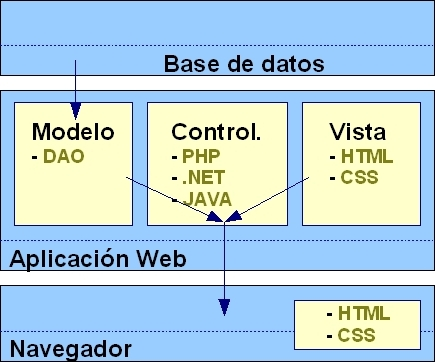
\includegraphics[width=0.7\textwidth]{imagenes/mvc.jpg}%ext=pdf,jpg,png
\caption{Patrón de diseño MVC}
\label{contexto:figura}
\end{figure}

\begin{itemize} 

\item \textbf{Modelo} es el responsable de:

\begin{itemize}
 \item Acceder a la capa de almacenamiento de datos. Lo ideal es que el modelo sea independiente del sistema de almacenamiento.
 \item Define las reglas de negocio (la funcionalidad del sistema).
 \item Lleva un registro de las vistas y controladores del sistema.
 \item Si estamos ante un modelo activo, notificará a las vistas los cambios que en los datos pueda producir un agente externo.
\end{itemize}

\item \textbf{Vista} es el responsable de:

\begin{itemize}
 \item Recibir datos del modelo y los muestra al usuario.
 \item Tienen un registro de su controlador asociado.ñ
 \item Pueden dar el servicio de Actualización, para que sea invocado por el controlador o por el modelo cuando es un modelo activo.\\
\end{itemize}


\item \textbf{Controlador:}

\begin{itemize}
 \item Recibir los eventos de entrada.
 \item Contiene reglas de gestión de eventos, estas acciones pueden suponer peticiones al modelo o a las vistas.\\
\end{itemize}

\end{itemize}

Aunque se pueden encontrar diferentes implementaciones de MVC, el flujo que sigue el control generalmente es el siguiente:

\begin{itemize}
  \item El usuario interactúa con la interfaz de usuario de alguna forma (por ejemplo, el usuario pulsa un botón, enlace, etc.)
  \item El controlador recibe (por parte de los objetos de la interfaz-vista) la notificación de la acción solicitada por el usuario. El controlador gestiona el evento que llega, frecuentemente a través de un gestor de eventos (handler) o callback.
  \item El controlador accede al modelo, actualizándolo, posiblemente modificándolo de forma adecuada a la acción solicitada por el usuario (por ejemplo, el controlador actualiza el carro de la compra del usuario). Los controladores complejos están a menudo estructurados usando un patrón de comando que encapsula las acciones y simplifica su extensión.
  \item El controlador delega a los objetos de la vista la tarea de desplegar la interfaz de usuario. La vista obtiene sus datos del modelo para generar la interfaz apropiada para el usuario donde se refleja los cambios en el modelo (por ejemplo, produce un listado del contenido del carro de la compra). El modelo no debe tener conocimiento directo sobre la vista. Sin embargo, el patrón de observador puede ser utilizado para proveer cierta indirección entre el modelo y la vista, permitiendo al modelo notificar a los interesados de cualquier cambio. Un objeto vista puede registrarse con el modelo y esperar a los cambios, pero aun así el modelo en sí mismo sigue sin saber nada de la vista. El controlador no pasa objetos de dominio (el modelo) a la vista aunque puede dar la orden a la vista para que se actualice. Nota: En algunas implementaciones la vista no tiene acceso directo al modelo, dejando que el controlador envíe los datos del modelo a la vista.
  \item La interfaz de usuario espera nuevas interacciones del usuario, comenzando el ciclo nuevamente.
\end{itemize}

\subsection{SISTEMA DE CONTROL DE VERSIONES}

Une definicion basica para entender de versión, revisión o edición de un producto, es el estado en el que se encuentra en un momento dado en su desarrollo o modificación.\\

Por lo tanto se llama control de versiones a la gestión de los diversos cambios que se realizan sobre los elementos de algún producto o una configuración del mismo. Los sistemas de control de versiones facilitan la administración de las distintas versiones de cada producto desarrollado, así como las posibles especializaciones realizadas (por ejemplo, para algún cliente específico).\\

El control de versiones se realiza principalmente en la industria informática para controlar las distintas versiones del código fuente. Sin embargo, los mismos conceptos son aplicables a otros ámbitos como documentos, imágenes, sitios web, etcétera.\\

Aunque un sistema de control de versiones puede realizarse de forma manual, es muy aconsejable disponer de herramientas que faciliten esta gestión (CVS, Subversion, SourceSafe, ClearCase, Darcs, Bazaar, Plastic SCM, Git, Mercurial, etc.).\\

La facilidad que estos sistemas aportan son:
\begin{itemize}
\item permite a los programadores comunicar fácilmente su trabajo a otros.
\item le permite a un equipo compartir el código.
\item mantener versiones separadas de “producción” que están siempre deployables.
\item permite el desarrollo simultáneo de diferentes características en el mismo código base.
\item mantiene la pista de todas las versiones viejas de archivos.
\item previene que se sobrescriba trabajo.
\end{itemize}

Conflicto en la utilizacion de los sitemas de control de versiones:
\begin{itemize}
  \item los usuarios X e Y despliegan versiones del archivo A en que las líneas n1 hasta n2 son comunes.
  \item el usuario X envía cambios entre las líneas n1 y n2 al archivo A
  \item el usuario Y no actualiza el archivo A tras el envío del usuario X
  \item el usuario Y realiza cambios entre las líneas n1 y n2
  \item el usuario Y intenta posteriormente enviar esos cambios al archivo A 
\end{itemize}

El sistema es incapaz de fusionar los cambios. El usuario Y debe resolver el conflicto combinando los cambios, o eligiendo uno de ellos para descartar el otro.

\subsubsection{CLASIFICACIÓN}

\begin{itemize}
\item \textbf{CENTRALIZADOS :}\\
Se basan en un repositorio único central con toda la información de cambios realizados el cual es accesible por todos los desarrolladores.\\
al haber un solo repositorio, este es el encargado del manejo de las ramas, quedando todos dentro de este. Están basados en una linea de tiempo, necesitan un servidor con funcionamiento de tiempo completo y con conexión permanente
configurado con algún sistema de autentificacion y permisos, por tal motivo la configuración suele ser mas compleja, según la necesidad. 
una de las desventajas mayores que representa es la dependencia de conexión con el servidor, ya que toda la información es manejada por el repositorio.\\
Generalmente hay dos tipos el Lock-Modify-Unlock y los que usan el modelo Copy-Modify-Merge. el primero es el mas simple y limitado, y consiste en que cada vez que un usuario quiere editar un archivo, este se bloquea y por lo tanto no puede ser
modificado por nadie mas, hasta que el usuario lo desbloquee. El segundo modelo propone lo siguiente: se hace una copia del estado actual del repositorio, se modifica y se aplica el conjunto de cambios al repositorio central haciendo un merge\footnote{Accion conocida en todo sistema de control de versiones, que cumple la accion de fusionar codigo.}, El cual es una forma de trabajo mas conveniente.
\item \textbf{DISTRIBUIDOS :}\\
Carece de un punto central de desarrollo por tanto los repositorios están distribuidos y descentralizados en diferentes maquinas que pueden o no ser independientes entre si, y 
técnicamente no hay ninguno mas importante que otro. Esto trae bastante beneficios al desarrollar, dado que cada desarrollador tenga su repositorio propio sobre el cual trabaje de una forma independiente, y periódicamente se pongan en común los trabajos de todos en algún repositorio convenido a tal efecto.

Esto da una serie de ventajas al sistema centralizado, como son:
  \begin{itemize}
    \item Disponer de forma distribuida de la información del repositorio al completo, tanto de forma local, como a través de los demás componentes del grupo.
    \item Cada cambio se va replicando entre los demás equipos distribuidos, a modo de que puedan emplear esos datos y actualizarlos en sus sistemas.
    \item El sistema de control de versiones distribuido ha sido pensado con la forma de trabajo basada en ramas, unión central en una sola versión (trunk) y liberaciones (o tags). Con lo que cada rama puede identificarse como cada copia distribuida que se use.
    \item Una máquina servidora puede emplearse, al estar siempre conectada, como otro punto de sincronización, con la ventaja de que, aunque cayera, mientras haya más miembros conectados, el sistema siempre se mantiene activo y con buen ancho de banda.
  \end{itemize}
 
\end{itemize}

\subsection{MICROBLOG}

Los blogs, como los conocemos actualmente, son espacios diseñados para que los navegantes de Internet puedan escribir libremente temas de cualquier índole, pueden ser aspectos de su vida diaria, pequeños post sobre sucesos extraños, denuncias, etcétera; la capacidad de expresar y escribir se limita al autor del blog.\\

El microblog puede considerarse como el hermano menor de los blogs; a diferencia de éstos, los caracteres son muy limitados, entre 100 y 150. 


\subsection{SERVICIOS WEB}

Existen múltiples definiciones sobre lo que son los Servicios Web, lo que muestra su complejidad a la hora de dar una adecuada definición que englobe todo lo que son e implican. Una posible sería hablar de ellos como un conjunto de aplicaciones o de tecnologías con capacidad para interoperar en la Web. Estas aplicaciones o tecnologías intercambian datos entre sí con el objetivo de ofrecer unos servicios. Los proveedores ofrecen sus servicios como procedimientos remotos y los usuarios solicitan un servicio llamando a estos procedimientos a través de la Web.\\

Estos servicios proporcionan mecanismos de comunicación estándares entre diferentes aplicaciones, que interactúan entre sí para presentar información dinámica al usuario. Para proporcionar interoperabilidad y extensibilidad entre estas aplicaciones, y que al mismo tiempo sea posible su combinación para realizar operaciones complejas, es necesaria una arquitectura de referencia estándar.\\


\subsection{WEB API}
Una API es una interfaz de programación de aplicaciones (del inglés API: Application Programming Interface). Es un conjunto de rutinas que provee acceso a funciones de un determinado software.\\

Son publicadas por los constructores de software para permitir acceso a características de bajo nivel o propietarias, detallando solamente la forma en que cada rutina debe ser llevada a cabo y la funcionalidad que brinda, sin otorgar información a cerca de como se lleva a cabo la tarea. Son utilizadas por los programadores para construir sus aplicaciones sin necesidad de volver a programar funciones ya hechas por otros, reutilizando código que se sabe que está probado y que funciona correctamente.\\

En la web las API's también son sinónimos de Web Service, las API's son publicadas por sitios para brindar la posibilidad de realizar alguna acción o acceder a alguna característica o contenido que el sitio provee. 

Una API puede ser:

\begin{itemize}
 \item \textbf{DEPENDIENTE DEL LENGUAJE:}\\ Que es disponible solo por un lenguaje de programación dado, usando la sintaxis y elementos de ese lenguaje para hacer conveniente el uso del API en esa petición.
 \item \textbf{INDEPENDIENTE DEL LENGUAJE:}\\ Que puede ser llamado por un gran numero de de lenguajes de programación. Esta es una característica de un servicio al estilo de la API que no está vinculada a un determinado proceso o sistema y está disponible como una llamada a procedimiento remoto(RPC Remote ).
\end{itemize}

\subsection{LINEA DE COMANDOS}

Un intérprete de órdenes, intérprete de línea de órdenes, intérprete de comandos, terminal, consola, shell o su acrónimo en inglés CLI (por Command Line Interface) es un programa informático que actúa como interfaz de usuario para comunicar al usuario con el sistema operativo mediante pantalla completa o ventana que espera órdenes escritas por el usuario en el teclado (ej. cd directorio), los interpreta y los entrega al sistema operativo para su ejecución. La respuesta del sistema operativo se muestra al usuario en la misma ventana. A continuación, el programa shell queda esperando más instrucciones. Se interactúa con la información de la manera más sencilla posible, sin gráficas, sólo el texto crudo.\\

Por extensión, también se llama intérprete de comandos a algunas interfaces de programas (mayores) que comunican al usuario con el software o al cliente de un servidor como, por ejemplo, bancos de datos (MySQL, Oracle) u otros programas (openSSL, FTP), etc.\\

Dada la importancia de esta herramienta, existe ya desde los comienzos de la computación. Existen, para diversos sistemas operativos, para diversos hardware, y con diferente funcionalidad. Suelen incorporar características tales como control de procesos, redirección de entrada/salida, listado y lectura de ficheros, protección, comunicaciones y un lenguaje de órdenes para escribir programas por lotes(scripts o guiones).\\

Su contraparte es la interfaz gráfica de usuario que ofrece una estética mejorada a costa de mayor consumo de recursos computacionales, una mayor vulnerabilidad por complejidad y, en general, una reducción en la funcionalidad ofrecida.\\

\begin{figure}[htb]
\centering
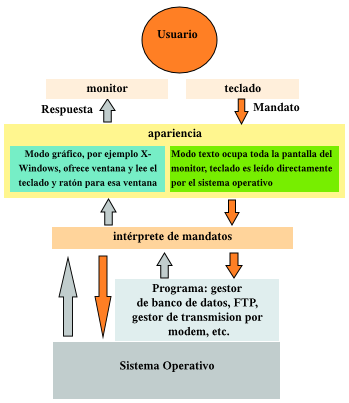
\includegraphics[width=0.6\textwidth]{imagenes/lineaDeComandos.png}%ext=pdf,jpg,png
\caption{... esquema de elementos involucrados en una linea de ordenes ...}
\label{contexto:figura}
\end{figure}


%\end{document}
